%%%%%%%%%%%%%%%%%%%%%%%%%%%%%%%%%%%%%%%%%
% Masters/Doctoral Thesis 
% LaTeX Template
% Version 1.43 (17/5/14)
%
% This template has been downloaded from:
% http://www.LaTeXTemplates.com
%
% Original authors:
% Steven Gunn 
% http://users.ecs.soton.ac.uk/srg/softwaretools/document/templates/
% and
% Sunil Patel
% http://www.sunilpatel.co.uk/thesis-template/
%
% License:
% CC BY-NC-SA 3.0 (http://creativecommons.org/licenses/by-nc-sa/3.0/)
%
% Note:
% Make sure to edit document variables in the Thesis.cls file
%
%%%%%%%%%%%%%%%%%%%%%%%%%%%%%%%%%%%%%%%%%

%----------------------------------------------------------------------------------------
%	PACKAGES AND OTHER DOCUMENT CONFIGURATIONS
%----------------------------------------------------------------------------------------

\documentclass[11pt, oneside]{Thesis} % The default font size and one-sided printing (no margin offsets)

\graphicspath{{Pictures/}} % Specifies the directory where pictures are stored

\usepackage[square, numbers, comma, sort&compress]{natbib} % Use the natbib reference package - read up on this to edit the reference style; if you want text (e.g. Smith et al., 2012) for the in-text references (instead of numbers), remove 'numbers' 
\hypersetup{urlcolor=blue, colorlinks=true} % Colors hyperlinks in blue - change to black if annoying
\title{\ttitle} % Defines the thesis title - don't touch this

\begin{document}

\frontmatter % Use roman page numbering style (i, ii, iii, iv...) for the pre-content pages

\setstretch{1.3} % Line spacing of 1.3

% Define the page headers using the FancyHdr package and set up for one-sided printing
\fancyhead{} % Clears all page headers and footers
\rhead{\thepage} % Sets the right side header to show the page number
\lhead{} % Clears the left side page header

\pagestyle{fancy} % Finally, use the "fancy" page style to implement the FancyHdr headers

\newcommand{\HRule}{\rule{\linewidth}{0.5mm}} % New command to make the lines in the title page

% PDF meta-data
\hypersetup{pdftitle={\ttitle}}
\hypersetup{pdfsubject=\subjectname}
\hypersetup{pdfauthor=\authornames}
\hypersetup{pdfkeywords=\keywordnames}

\newcommand{\Tau}{\mathcal{T}}

%----------------------------------------------------------------------------------------
%	TITLE PAGE
%----------------------------------------------------------------------------------------

\begin{titlepage}
\begin{center}

\textsc{\LARGE \univname}\\[1.5cm] % University name
\textsc{\Large Bachelor Thesis}\\[0.5cm] % Thesis type

\HRule \\[0.4cm] % Horizontal line
{\huge \bfseries \ttitle}\\[0.4cm] % Thesis title
\HRule \\[1.5cm] % Horizontal line
 
\begin{minipage}{0.4\textwidth}
\begin{flushleft} \large
\emph{Author:}\\
{\authornames} % Author name - remove the \href bracket to remove the link
\end{flushleft}
\end{minipage}
\begin{minipage}{0.4\textwidth}
\begin{flushright} \large
\emph{Supervisor:} \\
\href{https://www.telematik.uni-freiburg.de/aboutus/staff/staff?person=Lange_A}{\supname} % Supervisor name - remove the \href bracket to remove the link  
\end{flushright}
\end{minipage}\\[3cm]
 
\large \textit{A thesis submitted in fulfilment of the requirements\\ for the degree of \degreename}\\[0.3cm] % University requirement text
\textit{in the}\\[0.4cm]
\groupname\\\deptname\\[2cm] % Research group name and department name
 
{\large \today}\\[4cm] % Date
%\includegraphics{Logo} % University/department logo - uncomment to place it
 
\vfill
\end{center}

\end{titlepage}

%----------------------------------------------------------------------------------------
%	DECLARATION PAGE
%	Your institution may give you a different text to place here
%----------------------------------------------------------------------------------------

\Declaration{

\addtocontents{toc}{\vspace{1em}} % Add a gap in the Contents, for aesthetics

I, \authornames, declare that this thesis titled, '\ttitle' and the work presented in it are my own. I confirm that:

\begin{itemize} 
\item[\tiny{$\blacksquare$}] This work was done wholly or mainly while in candidature for a research degree at this University.
\item[\tiny{$\blacksquare$}] Where any part of this thesis has previously been submitted for a degree or any other qualification at this University or any other institution, this has been clearly stated.
\item[\tiny{$\blacksquare$}] Where I have consulted the published work of others, this is always clearly attributed.
\item[\tiny{$\blacksquare$}] Where I have quoted from the work of others, the source is always given. With the exception of such quotations, this thesis is entirely my own work.
\item[\tiny{$\blacksquare$}] I have acknowledged all main sources of help.
\item[\tiny{$\blacksquare$}] Where the thesis is based on work done by myself jointly with others, I have made clear exactly what was done by others and what I have contributed myself.\\
\end{itemize}
 
Signed:\\
\rule[1em]{25em}{0.5pt} % This prints a line for the signature
 
Date:\\
\rule[1em]{25em}{0.5pt} % This prints a line to write the date
}

\clearpage % Start a new page

%----------------------------------------------------------------------------------------
%	QUOTATION PAGE
%----------------------------------------------------------------------------------------

\pagestyle{empty} % No headers or footers for the following pages

\null\vfill % Add some space to move the quote down the page a bit

\textit{``Companies spend millions of dollars on firewalls, encryption and secure access devices, and it’s money wasted, because none of these measures address the weakest link in the security chain."}

\begin{flushright}
Kevin Mitnick
\end{flushright}

\vfill\vfill\vfill\vfill\vfill\vfill\null % Add some space at the bottom to position the quote just right

\clearpage % Start a new page

%----------------------------------------------------------------------------------------
%	ABSTRACT PAGE
%----------------------------------------------------------------------------------------

\addtotoc{Abstract} % Add the "Abstract" page entry to the Contents

\abstract{\addtocontents{toc}{\vspace{1em}} % Add a gap in the Contents, for aesthetics

The Thesis Abstract is written here (and usually kept to just this page). The page is kept centered vertically so can expand into the blank space above the title too\ldots
}

\clearpage % Start a new page


%----------------------------------------------------------------------------------------
%	LIST OF CONTENTS/FIGURES/TABLES PAGES
%----------------------------------------------------------------------------------------

\pagestyle{fancy} % The page style headers have been "empty" all this time, now use the "fancy" headers as defined before to bring them back

\lhead{\emph{Contents}} % Set the left side page header to "Contents"
\tableofcontents % Write out the Table of Contents

\lhead{\emph{List of Figures}} % Set the left side page header to "List of Figures"
\listoffigures % Write out the List of Figures

\lhead{\emph{List of Tables}} % Set the left side page header to "List of Tables"
\listoftables % Write out the List of Tables

%----------------------------------------------------------------------------------------
%	THESIS CONTENT - CHAPTERS
%----------------------------------------------------------------------------------------

\mainmatter % Begin numeric (1,2,3...) page numbering

\pagestyle{fancy} % Return the page headers back to the "fancy" style

% Include the chapters of the thesis as separate files from the Chapters folder
% Uncomment the lines as you write the chapters

% Chapter Template

\chapter{Einleitung} % Main chapter title

\label{Chapter1} % Change X to a consecutive number; for referencing this chapter elsewhere, use \ref{ChapterX}

\lhead{Chapter 1. \emph{Einleitung und Motivation}} % Change X to a consecutive number; this is for the header on each page - perhaps a shortened title

%----------------------------------------------------------------------------------------
%	SECTION 1
%----------------------------------------------------------------------------------------

\section{Motivation}

Um Sicherheit in Unternehmen gewährleisten zu können, reicht es nicht aus, in teure Software zu investieren, die das Unternehmen gegen externe Angriffe absichert. Ein nicht zu unterschätzender Teil der Bedrohung befindet sich im Inneren des Unternehmens. Angestellte können ihre Position und ihr Wissen ausnutzen, um sich oder Anderen Vorteile zu verschaffen. Es müssen aber nicht immer betrügerische Absichten hinter der Handlung eines Angestellten stehen. Auch menschliches Versagen kann bei dem Unternehmen Schäden verursachen. Das einfachste Konzept, um zu verhindern, dass Angestellte internen Betrug oder Fehler begehen, ist das \textit{Separation of Duty} (\textbf{SOD}) Prinzip  \cite{SOD} \cite{SOD2}. Dabei werden kritische Aufgaben in kleinere Teile zerlegt, die nicht von einer einzigen Person ausgeführt werden dürfen. Somit wird ein gewisses Maß an Kontrolle geboten \footnote{Das Konzept versagt natürlich, wenn sich alle beteiligten Personen gemeinsam dazu entschließen, einen Betrug zu begehen.}. Jedoch beziehen sich die meisten Konzepte auf Aufgaben aus derselben Instanz eines Prozesses. Neuere Forschungsergebnisse \cite{warner_inter_instance} \cite{instance_spanning} weisen darauf hin, das dies nicht ausreicht, und man ebenfalls Einschränkungen auf Aufgaben definieren muss, die aus verschiedenen Prozessinstanzen stammen.

Ein Prozess (Arbeitsablauf) in einem Unternehmen besteht aus mehreren, in sich abgeschlossenen Aufgaben. Diesen Aufgaben werden Rollen zugewiesen, die potentiell dazu berechtigt sind, die Aufgabe auszuführen. Jeder Mitarbeiter besitzt ebenfalls eine potentialle Menge an Rollen, in denen er agieren kann. Sobald ein Mitarbeiter in einer authorisierten Rolle eine Aufgabe annimt, kann sie nur von ihm durchgeführt werden \footnote{Es gibt auch die Möglichkeit, Aufgaben wieder abzugeben oder an einen anderen Mitarbeiter weiterzuleiten.}.

Abbildung \ref{fig:WorkflowEinleitung} stellt eine schematische Darstellung der Aufgaben in einer Bank dar, nachdem ein Kunde einen Kreditwunsch geäußert hat.

\begin{figure}[ht]
	\centering
  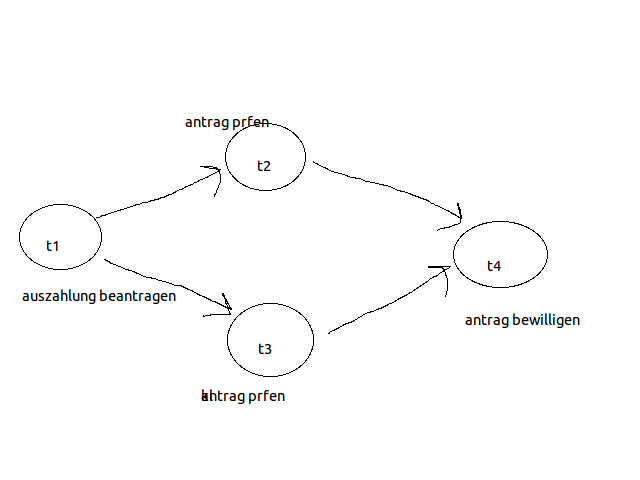
\includegraphics[width=0.9\textwidth]{Figures/Workflow}
	\caption{Arbeitsablauf in einer Bank, nachdem ein Kreditantrag eingegangen ist.}
	\label{fig:WorkflowEinleitung}
\end{figure}

Sobald ein Kreditantrag bei der Bank eingeht, muss dieser geprüft werden. Je nach Ergebnis der Prüfung, wird der Antrag entweder bewilligt oder abgelehnt. In jedem Fall muss der Kunde wieder kontaktiert werden.
Da es nicht erwünscht ist, dass der selbe Mitarbeiter, der den Antrag aufnimmt, ihn auch prüft, wird hier das \textit{Separation of Duty Prinzp} angewendet. Im einfachsten Fall würde der Prüfer die Fehler oder Falschangaben im Antrag entdecken und ihn zurückweisen. Ein schwierigeres Szenario ist, wenn sich zwei Angestellte absprechen und sich gegenseitig ihre Anträge bewilligen. Ein \textit{SOD} Modell, welches jeden Arbeitsablauf für sich betrachtet, würde diesen Betrug nicht erkennen. Es wird eine Lösung benötigt, auch Einschränkungen zwischen mehreren Instanzen eines Arbeitsablaufs zu definieren. Um den Schaden gering zu halten, könnte man verbieten, dass zwei Mitarbeiter in mehr als drei Arbeitsabläufen gemeinsam an T1 und T2 arbeiten.



%-----------------------------------
%	Ziel der Arbeit
%-----------------------------------

\section{Ziel der Arbeit}

Ziel der Arbeit ist es, eine Definitionssprache zu entwickeln, die es ermöglicht, Einschränkungen und Regeln zur Ausführung von Aufgaben durch bestimmte Angestellte sowohl innerhalb von Prozessinstanzen als auch zwischen mehreren Instanzen zu definieren. Dazu muss untersucht werden, welche Arten von Einschränkungen und Regeln es gibt und wie die Spannweite einer Regel definiert werden kann. Anschließend wird ein Modelchecker entwickelt, der \textit{Eventlogs} auf die Einhaltung dieser Regeln untersucht.



%-----------------------------------
%	AUFBAU DER ARBEIT
%-----------------------------------

\section{Aufbau der Arbeit}
Folgende Konventionen werden hier verwendet:\\
\textit{kursive Begriffe  bezeichnen Fachbegriffe}\\
\textbf{Definitionen und Abkürzungen werden beim ersten Vorkommen fett geschrieben}\\
\texttt{Blockschrift kennzeichnet Pseudocode, Klassennamen, Code,...}\\

Diese Arbeit setzt ein elementares Verständnis von Logik und logischer Programmierung voraus, da hier nicht näher darauf eingegangen wird.

In Kapitel 2 wird einerseits ein Überblick über die Grundlagenliteratur gegeben als auch verwandte Arbeit vorgestellt. Dabei wird kurz darauf eingegangen, inwiefern sich diese Arbeit von den Anderen unterscheidet. In Kapitel 3 werden wichtige Begriffe erläutert. In Kapitel 4 widmen wir uns der  Herleitung von Einschränkungen und der Definition einer entsprechenden Grammatik. Diese wird in Kapitel 5 in ein Programm integriert, welches Event Logs auf die Verletzung von Einschränkungen prüft. Dazu wird der Algorithmus vorgestellt und der Aufbau des Programms vorgestellt. In Kapitel 6 wird ein Beispiel zur Funktionsweise des Programms vorgestellt. Letztendlich wird die Arbeit in Kapitel 7 mit ein paar abschließenden Bemerkungen beendet.


% Chapter Template

\chapter{Theoretische Grundlagen} % Main chapter title

\label{Chapter2} % Change X to a consecutive number; for referencing this chapter elsewhere, use \ref{ChapterX}

\lhead{Chapter 2. \emph{Introduction}} % Change X to a consecutive number; this is for the header on each page - perhaps a shortened title

%-----------------------------------
%	SECTION
%-----------------------------------
\section{Erklärung der Begriffe}
 In diesem Kapitel werden wichtige Begriffe vorgestellt, die im Verlauf der weiteren Arbeit von Bedeutung sind.

%-----------------------------------
%	WORKFLOW
%-----------------------------------
\subsection{Workflow}

Bild zu Workflow UML
Ein Workflow ist eine definierte Abfolge von abgeschlossenen Arbeitsaufgaben, den Tasks. 

TODO: suche nach einer offiziellen Definition von workflows

%-----------------------------------
%	TASKS
%-----------------------------------
\subsection{Tasks}

Tasks sind Aufgaben, die in sich abgeschlossen sind. Sie besitzen 3 verschiedene Zustände: Assigned, Started und Completed welche durch Events getriggert werden. Das MXML Modell unterstützt 13 verschiedene Events, die sich in ihrer Bennenung bei den einzelnen Programmen unterscheiden können. Events können auch feiner gegliedert sein, bzw es kann auch sein, dass nur eine Teilmenge davon verwendet wird. In dieser Arbeit gehen wir davon aus, dass es folgende Events gibt: started, assigned, completed, ...

\begin{figure}[ht]
	\centering
  \includegraphics[width=0.9\textwidth]{"Figures/Task Events"}
	\caption{Tasks und Events}
	\label{fig2}
\end{figure}

%-----------------------------------
%	AUTHORISIERUNG
%-----------------------------------
\subsection{Authorisierung}

%-----------------------------------
%	ROLLENMODELL
%-----------------------------------
\subsection{Rollenmodell}

%-----------------------------------
%	ZEITMODELL
%-----------------------------------
\subsection{Zeitmodell}

%-----------------------------------
%	Event Logs
%-----------------------------------
\subsection{Event Logs}

EventLogs sind Abbildungen von Workflows. Ein EventLog kann durchaus unvollständig sein bzw Fehler beinhalten.

Das in dieser Thesis verwendete Format für Event Logs ist der Standard MXML

\begin{figure}[ht]
	\centering
  \includegraphics[width=0.9\textwidth]{"Figures/mxml"}
	\caption{MXML Modell}
	\label{fig:mxml}
\end{figure}


\begin{table}[h]
  \centering
  \begin{tabular}{|c|c|c|c|c|c|}
  caseID & Task & User & Role & Timestamp & EventType\\
  \hline
  0 & Approach check &'Mark' &'Admin' &1999-12-13T12:22:15 & start\\
  0 & Pay check & 'Theo' &'Azubi' &1999-12-13T12:22:16 & start\\
  1 & Approach check &'Lucy' & 'Azubi' &1999-12-13T12:22:17 &start\\
  1 & Pay check &'Mark' & 'Admin' &1999-12-13T12:22:18 & abort\\
  0 & Revoke check & 'Theo' & 'Clerk' & 1999-12-13T12:22:19 & start
  \end{tabular}
Das ist nur ein Auszug und kein vollständiger Log. Es können auch weitere Daten vorhanden sein, die hier nicht dargestellt werden.
  \caption{Beispiel Log Einträge. }
  \label{tab:examplelog}
\end{table}


%-----------------------------------
%	Definition Constraints
%-----------------------------------
\subsection{Definition Constraints}

%-----------------------------------
%	Security policy
%-----------------------------------
\subsection{Schutzziele}
Die von Accorsi nehmen. Später darauf eingehen, was eingehalten wurde. Bzw schon bei Definition von Constraints darauf eingehen.





 
% Chapter Template

\chapter{Verwandte Arbeit} % Main chapter title

\label{Chapter3} % Change X to a consecutive number; for referencing this chapter elsewhere, use \ref{ChapterX}

\lhead{Chapter 3. \emph{Introduction}} % Change X to a consecutive number; this is for the header on each page - perhaps a shortened title

%-----------------------------------
%	SECTION
%-----------------------------------

\section{Related work}


\subsection{Geschichte}
Chinese Wall Modell Bewer/ Nash\\
Business Rules und Auditierung ??
Um die Zuverlässigkeit von Abläufen zu gewährleisten, wird schon lange Auditierung betrieben. Ursprünglich ging es darum, den korrekten Ablauf nachzuweisen. Man kann damit aber auch die zulässige Ausführung von Ereignissen prüfen.
\subsection{Heute}
Übergang zu Inter/instance Constraints
Heute: verschiedene Forschungszweige: TBAC, Inter-Instance Constraints
Allgemein eher den Inhalt auswerten, statt eine Liste von verwandten Arbeiten anzugeben
Arten Unterscheiden, wie man Constraints spezifizieren kann
Als logische Prädikate, GL4
Welche Constraint-Richtungen werden behandelt?
ZB nur Entailment, Cardinality. 
\subsection{warner inter-Instance}
Diese Arbeit bezieht sich hauptsächlich auf die Arbeit von Warner und Atluri \cite{warner_inter_instance}.
In dieser Arbeit wird der theoretische Ansatz von Bertino et al. um inter instance constraints erweitert und ist der Ausgangspunkt meiner Arbeit. Allerdings gehen sie davon aus, dass die Constraints für Authorisierungszwecke gedacht sind, und unterscheiden deswegen zwischen statischer Analyse zur Entwurfszeit und dynamischer Analyse während des Ablaufs. Bei der dynamischen Analyse werden die Informationen nach jeder Aktion  aktualisiert und unter Umständen die Liste von verbotenen Nutzern / Rollen angepasst.
Da ich Auditierung benutze, wird statically checked weggelassen und weitere Regeln, die zur Laufzeit nötig sind.\\
Das Paper ist allerdings nur ein theoretischer Ansatz und behandelt zB die verschiedenen Eventtypen nicht ausreichen. Des weiteren wird nicht darauf eingegangen, was passiert, wenn  manche Informationen fehlen.
\subsection{leitner instance-spanning}
Hat ein Framework entwickelt.
\subsection{tan consistency}
Es geht eher um die Prüfung auf Konsistenz, es werden aber globale Constraints erwähnt.




\subsection{ProM - SCIFFchecker}
Sciff wurde von Marco Alberti, Federico Chesani und Marco Gavanelli im Rahmen des SOCS Projekts entwickelt. Es arbeitet ebenfalls mit Prolog, kann aber keine Inter Instance Constraints.



 
% Chapter Template

\chapter{Grundlagen} % Main chapter title

\label{Chapter4} % Change X to a consecutive number; for referencing this chapter elsewhere, use \ref{ChapterX}

\lhead{Chapter 4. \emph{Grundlagen}} % Change X to a consecutive number; this is for the header on each page - perhaps a shortened title

%-----------------------------------
%	THEORIE
%-----------------------------------

\section{Grundlagen und Definitionen}
In diesem Kapitel werden wichtige Begriffe vorgestellt, die im Verlauf der weiteren Arbeit von Bedeutung sind.

%-----------------------------------
%	WORKFLOW CASES
%-----------------------------------
\subsection{Prozess Schemata und Instanzen}

Ein Prozessschema \textbf{W = $\{T,D\}$} mit n $\in \mathbb{N}$ ist eine Menge von Aktivitäten \textbf{T = $\{t_1,t_2,...,t_n\}$} und einer Menge \textbf{D} von Abhängigkeiten, welche bestimmen, in welcher Reihenfolge die einzelnen Aktivitäten ausgeführt werden bzw von welchen Parametern abhängt, ob sie ausgeführt werden müssen, oder nicht. Die Menge der Aktivitäten muss mindestens eine Startaktivität haben, kann aber mehrere terminierende Aktivitäten beinhalten, die gleichberechtigt den Prozess abschließen.
$t_{ij}$ bezeichnet hierbei die Aktivität $t_j$ aus dem Prozessschema $W_i$. \\

\begin{figure}[ht]
	\centering
  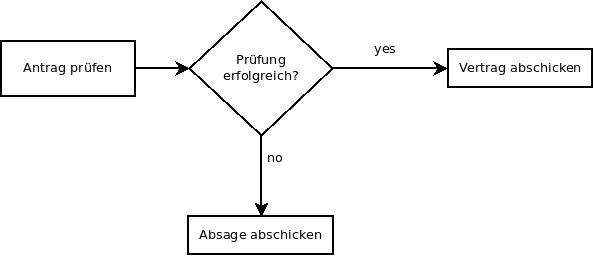
\includegraphics[width=0.7\textwidth]{Figures/sampleW}
	\caption{einfaches Beispiel eines Prozessschemas}
Ein einfaches Beispiel für das Schema eines Prozesses mit einem Start und zwei finalen Aktivitäten.In Abhängigkeit davon, welcher Wert für x berechnet wird, wird der Prozess entweder sofort abgebrochen, oder es werden weitere Aktivitäten ausgeführt.
	\label{fig2}
\end{figure}

Ein Prozessschema kann mehrere Instanzen besitzen, die mit \textbf{W$_i^k$} gekennzeichnet werden.
Eine Prozessinstanz $W_i^k$ ist eine Menge von Instanzen $T_i^k$ der zugehörigen Aktivitäten. Dabei ist $|T_i| \subseteq |T|$ eine Teilmenge aller möglichen Aktivitäten des zugehörigen Schemas, da einzelne Aktivitäten unter Umständen aufgrund der Abhängigkeiten nicht ausgeführt werden müssen.


%-----------------------------------
%	ACTIVITIES TASKS
%-----------------------------------
\subsection{Aktivitäten}
\label{sec:activities}
Eine Aktivität ist ein atomares Event, dh. eine in sich abgeschlossene Aufgabe im Kontext eines Prozesses. Sie haben eine definierte Menge von potentiellen Rollen und Nutzern, die die Erlaubnis besitzen, diese Aufgabe auszuführen. Sobald sie einem Nutzer zugewiesen wurde, kann kein weiterer Nutzer mehr die Aufgabe annehmen. Das bedeutet, dass jede Aktivität einen eindeutigen Nutzer und eine eindeutige Rolle hat, welcher sie ausgeführt hat.

Des weiteren besitzen die Aktivitäten einen eindeutigen Zeitstempel $\tau$, zu dessen Zeitpunkt sie ausgeführt wurden. Diese Zeitstempel bestimmen eine Ordnung $<T, \leq>$. Es gilt nämlich $t_1 < t_2 $, wenn $t_1$ vor $t_2$ ausgeführt wurde, dh. timestamp($t_1$) $<$ timestamp($t_2$).

Aktivitäten besitzen 7 verschiedene Zustände: \textit{new, scheduled, assigned, active, suspended, completed, aborted}. Die Aktivitäten werden durch \textbf{Events} von einem Zustand in den nächsten geführt. Die Übergänge können sehr fein gegliedert sein oder sich nur auf elementare \textit{Events} beschränken. In dieser Arbeit wird von 12 \textit{Event}-Typen ausgegangen: \textit{schedule, assign, reassign, start, complete, resume, suspend, autoskip, manualskip, withdraw, ate\_abort, pi\_abort}.

\begin{figure}[ht]
	\centering
  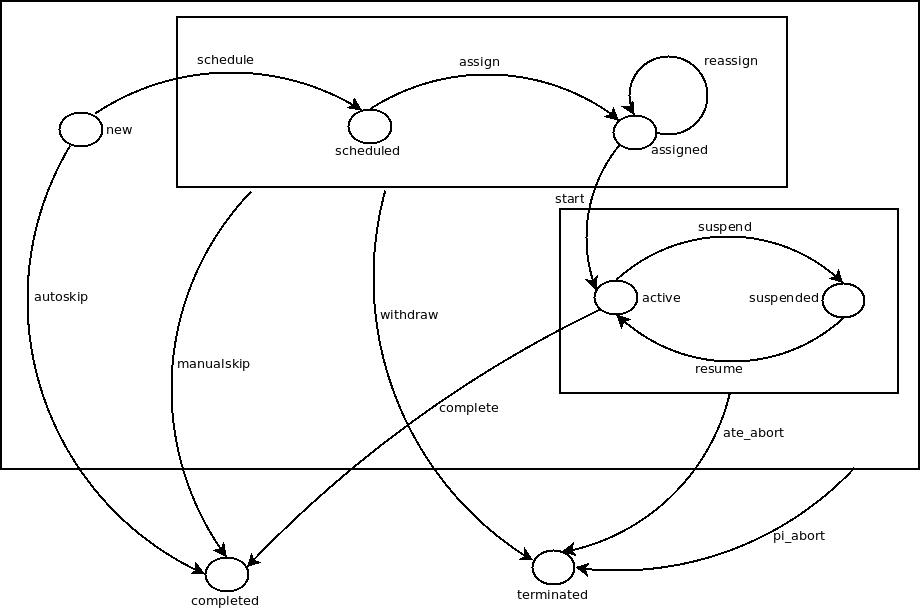
\includegraphics[width=0.9\textwidth]{Figures/Taskevents}
	\caption{Aktivitäten und Events}
Eine Aktivität und ihre möglichen Zustände. Der Startzustand ist \textit{new}. Die neue Aktivität kann entweder sofort verworfen werden oder wird einem Nutzer zugewiesen und gestartet. Es gibt die Möglichkeit, die Aufgabe einem anderen Nutzer zuzuweisen oder zu pausieren und wieder zu starten. Aus jedem Zustand heraus kann die Aktivität abgebrochen werden.
	\label{fig2}
\end{figure}
 

%-----------------------------------
%	ROLLENMODELL
%-----------------------------------
\subsection{Rollenmodell und Authorisierung}
Sei \textbf{T} = $\{t_1,t_2,...t_m\}$, $m\in\mathbb{N}$ eine Menge von Tasks, \textbf{R} = $\{r_1,r_2,...t_n\}$, $n\in\mathbb{N}$ eine Menge von Rollen, und \textbf{U} = $\{u_1,u_2,...u_l\}$,$l\in\mathbb{N}$ eine Menge von Usern.

\begin{figure}[ht]
	\centering
  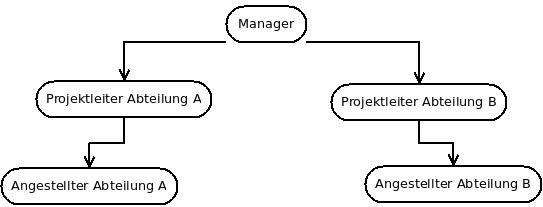
\includegraphics[width=0.9\textwidth]{Figures/Rollenmodell}
	\caption{Beispiel Rollenmodell}
	\label{fig:examplerolemodel}
\end{figure}

Eine \textbf{Authorisierung} ist eine Menge von potentiellen Nutzer und Rollen, denen es erlaubt ist, einen Task auszuführen. Eine Authorisierung besteht aus den Tupeln $$\textbf{TR} = (T\times R)$$ und $$\textbf{UR} = (U\times R)$$, welche eine n:m-Beziehung zwischen Tasks und Rollen, bzw zwischen Usern und Rollen kennzeichnen. Das bedeutet, dass User mit Rollen in der User-Rollen Beziehung assoziiert werden und Tasks mit Rollen in der Tast-Rollen Beziehung assoziiert werden.\\
Sei nun $$\textbf{R(t)} = \{r_m \in R: \exists(t_k, r_m) \in TR(t)\}$$
$$\textbf{U(t)} = \{u_n \in U: \exists(u_n, r_m) \in UR, r_m \in R(t)\}$$
Mit anderen Worten ist R(t) die Menge aller Rollen, die authorisiert sind, einen Task auszuführen und U(t) die Menge alles User, die authorisiert sind, einem Task zugeteilt zu werden.\\
Eine \textbf{Zuweisung} ist die konkrete Ausführung eines Tasks durch einen User.

Ein \textbf{hierarchisches Rollenmodell} ist eine geordnete Menge von Beziehungen zwischen Rollen $<R, \leq>$. Wenn $r_1, r_2 \in R$ und $r_1 < r_2$, dann dominiert die Rolle $r_2$ die Rolle $r_1$ in Bezug auf die organisatorische Rollenhierarchie. In Abb. \ref{fig:examplerolemodel} dominiert die Rolle "Projektleiter" die Rolle "Angestellter", das bedeutet, dass der "Projektleiter" alle Tasks ausführen darf, die der Rolle "Angestellter" zugeordnet wurde.
Die Rolle und all ihre Elternrollen bis zur Wurzel können einem Task zugewiesen werden.

\cite{wolter_modeling_of_TBAC_in_BPMN}

%-----------------------------------
%	ZEITMODELL
%-----------------------------------
\subsection{Zeitmodell}
Das Zeitmodell ist ein Tupel T = ($\Tau;\leq$).\\
$\Tau$ ist eine Menge von \textit{Zeitpunkten} $\tau$ und $\leq$ eine total Ordnung auf $\Tau$.
Ein \textit{Zeitinterval}$[\tau_a, \tau_b]$ ist eine Menge von Zeitpunkten $\tau \in \Tau$ mit $\tau_a \leq \tau \leq \tau_b$.
Ein Zeitinterval $\tau' = [\tau_a, \tau_b]$ wird als leer bezeichnet, falss $\tau_b \leq \tau_a$.

\textbf{TS} wird als die Menge aller Zeitpunkt Symbole wie 30.07.1999, 14:55 definiert und \textbf{TP} bezeichnet die Menge aller Zeitspannen wie 3 Tage 5 Stunden, 5 Monate. \textbf{TV} ... Variablen für Zeitpunkte TODO


\cite{warner_inter_instance}

%-----------------------------------
%	Event Logs
%-----------------------------------
\subsection{Event Logs}

EventLogs sind Abbildungen von Prozessen $W_i$ auf eine Teilmenge $E \subseteq W_i$. Ein EventLog kann durchaus unvollständig sein bzw Fehler beinhalten. Jedoch wird in dieser Arbeit von einer \textit{Closed World} ausgegangen, was bedeutet, dass eine Aktivität, die nicht geloggt wurde, auch nicht stattgefunden hat.


\begin{figure}[h!]
	\centering
  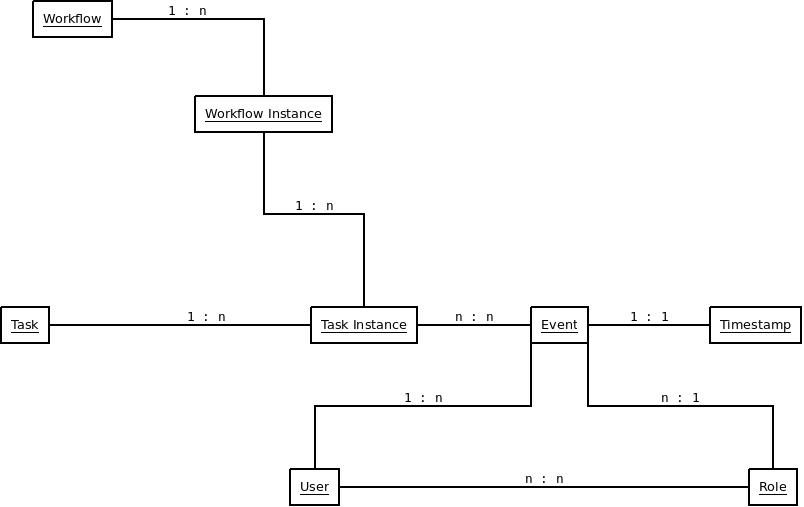
\includegraphics[width=0.9\textwidth]{Figures/WorkflowOntology}
	\caption{Ontologie eines Prozesses // TODO nochmal Beziehungen überdenken}
	\label{fig:ontology}
\end{figure}

// TODO Darstellung der additional Data, es ein bisschen verändern, damit man sieht, dass eine task von jedem element genau 1 hat

EventLogs repräsentieren die Instanzen eines Prozesses durch Auflistung der einzelnen Aktivitäten. In Tabelle \ref{tab:examplelog} wird ein exemplarischer Log dargestellt. Die \textit{caseID} kennzeichnet die Instanz des Prozesses, da ein Prozessschema mehrere Instanzen besitzen kann. Zu einer Prozessinstanz können mehrere Aktivitäten (hier \textbf{Task}) gehören, die jedoch einen eindeutigen Zeitstempel, Eventtypen, Nutzer und dessen Rolle haben. Zudem kann eine Aktivität beliebig viele zusätzliche Informationen besitzen, die in dieser Tabelle nur angedeutet werden.

\begin{table}[h!]
\footnotesize
  \centering
  \begin{tabular}{|c|c|c|c|c|c|c|}
  \hline
  caseID & Task & User & Role & Timestamp & EventType & DataAttributes\\
  \hline
  0 & Approach check &'Mark' &'Admin' &1999-12-13T12:22:15 & start&(amount, 3000)\\
  0 & Pay check & 'Theo' &'Azubi' &1999-12-13T12:22:16 & start&(amount, 3000Euro)\\
  1 & Approach check &'Lucy' & 'Azubi' &1999-12-13T12:22:17 &start&(customer, Max Muster)\\
  1 & Pay check &'Mark' & 'Admin' &1999-12-13T12:22:18 & abort&()\\
  0 & Revoke check & 'Theo' & 'Clerk' & 1999-12-13T12:22:19 & start&()\\
  \hline
  \end{tabular}
\\
Das ist nur ein Auszug und kein vollständiger Log. Es können auch weitere Daten vorhanden sein, die hier nicht dargestellt werden.
  \caption{Beispiel Log Einträge. }
  \label{tab:examplelog}
\end{table}



%-----------------------------------
%	Security policy
%-----------------------------------
\subsection{Schutzziele}

Um bestimmen zu können, welche Regeln und Einschränkungen für den Ablauf eines Prozesses notwendig sein könnten, muss zuletzt noch auf die Schutzziele von Unternehmen (besseres Wort) eingegangen werden.

Müller et al. \cite{mueller_accorsi} sammeln unter anderem\footnote{Ein weiteres Schutzziel ist "Data Integrity" und "Nutzungskontrolle", welches für diese Arbeit nicht relevant ist.} folgende Punkte:\\

\textbf{(1) Autorisierung}\\
Welche Subjekte bzw Rollen dürfen auf welche Ressourcen zugreifen? Da es in größeren Unternehmen komplex werden kann, wurde das Rollenmodell zur Vereinfachung entwickelt. \\
\textbf{(2) Nutzungskontrolle}\\
Regelt die Art der Nutzung. RWX, begrenzte Anzahl an Zugriffen, bzw Verpflichutung einer Löschoperation (weiteren, resultierenden Handlungen) nach Zugriff(Kontrollfluss)\\
\textbf{(3) Interessenskonflikt}\\
Unterbindung von unzulässiger Ausnutzung von insider-Wissen. Chinese Wall Modell.\\
\textbf{(4) Funktionstrennung}\\
Bestimmte Aufgaben dürfen nicht vom selben Subjekt, Rolle, Abteilung, ausgeführt werden. Unterbindung von kriminellen Handlungen und Betrug.\\
\textbf{(5) Aufgabenbindung}\\
Gegenteil von Funktionstrennung\\
\textbf{(6) Mehr-Augen-Kontrolle}\\
kritische Aktivität im Prozess darf nicht von einer einzelnen Person ausgeführt werden. Das wäre bei mir Cardinality Constraints, wenn eine Aktivität aus mehreren Tasks besteht.\\

// TODO: was kann man noch hinzufügen?



\section{Herleitung der Einschränkungen}


%-----------------------------------
%	Definition Constraints
%-----------------------------------

\subsection{Ein praktisches Beispiel mit vielen Einschränkungen}
\label{sec:exampleconstraints}

In diesem Kapitel werden verschiedene Arten von Einschränlungen und Regeln betrachtet.
Constraints sind Regeln bzw Einschränkungen, die aus dem Verlauf von vorhergehenden Tasks resultieren. Einschränkungen und Regeln werden hier synonym verwendet.
Einschränkungen haben den Zweck Betrug, aber auch menschliches Versagen zu verhindern.
Um sich ein besseres Bild von Einschränkungen zu machen, betrachten wir vor der eigentlichen Analyse ein Beispiel, welches im Verlauf der Arbeit auf die Einhaltung der Regeln untersucht wird.
Das folgende Beispiel wurde in leicht veränderter Form \cite{wolter_modeling_of_TBAC_in_BPMN} entnommen. // TODO stimmt das überhaupt?

Der Prozess in Abbildung \ref{fig:Workflow} stellt die Bearbeitungsschritte eines Kreditantrages in einer Bank dar. In (T1 - Antrag empfangen) müssen zuerst alle erforderlichen Daten des Kunden aufgenommen werden. Daraufhin muss der Antrag geprüft werden, wie zum Beispiel die Kreditwürdigkeit des Kunden (T2 - Antrag prüfen). Sollte der gewünschte Betrag des Kredites 100000 Euro übersteigen, muss der Antrag zur Sicherheit von einer weiteren Person geprüft werden (T3 - Antrag prüfen). Nun muss entweder ein Vertrag vorbereitet werden (T4) oder, falls die Prüfung negativ verlaufen ist, ein Schreiben vorbereitet werden, welches dan Antrag ablehnt (T5). Unabhängig von dem Ergebnis wird der Kunde zuletzt noch einmal kontaktiert (6).
\begin{figure}[ht]
	\centering
  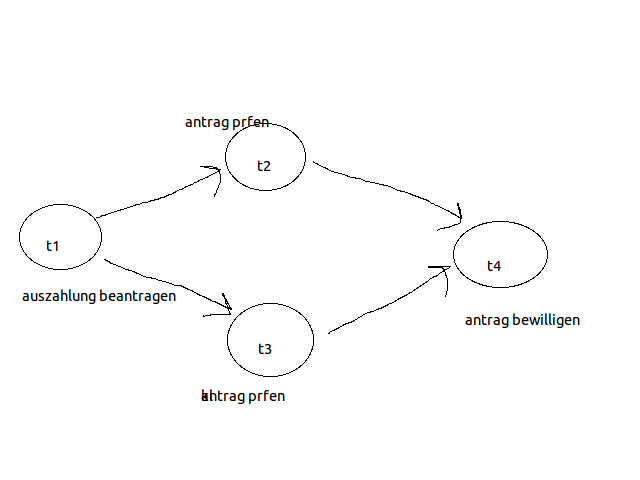
\includegraphics[width=0.9\textwidth]{Figures/Workflow}
	\caption{Bearbeitung eines Kreditantrags in der Bank}
	\label{fig:Workflow}
\end{figure}
\\
Um einen sicheren und reibungslosen Ablauf zu gewährleisten, werden folgende Anforderungen gestellt:

\begin{enumerate}
\item (Der Kontakt mit Kunden) T1 und T6 muss vom Kundenberater erledigt werden
\item Um den Kunden nicht zu lange warten zu lassen, sollte der Kunde spätestens 3 Tage nach erstem Kontakt über das Ergebnis informiert werden (timestamp(T6) $<$ timestamp(T1) + 3D)
\item Um zu verhindern, dass Fehler durch Überlastung passieren, darf jeder Mitarbeiter am Tag höchstens 100 Tasks bearbeiten.
\item Den Antrag annehmen (T1) und den Antrag prüfen(T2, T3) sollten von verschiedenen Personen erledigt werden (4 Augen Prinzip).
\item Ferner sollten auch die zwei Prüfungen von verschiedenen Mitarbeitern vollzogen werden. T3 muss durch den Bank Manager erfolgen.
\item Wenn ein Mitarbeiter 5x einem Task zugewiesen wird und ihn dann abbricht, darf er nicht mehr an dem Task arbeiten.
\item Es dürfen keine Anträge von Verwandten geprüft werden.
\item Es dürfen auch höchstens 3 mal Mitarbeiter an den Anträgen des jeweils anderen Verwandten arbeiten.
\item Ein Mitarbeiter darf bei dem selben Kunden höchstens Kredite bis 100000 Euro prüfen.
\item Es dürfen hochstens 3 mal die selben Personen an T2 und T3 arbeiten
\end{enumerate}


%
% Arten von Constraints
%
\subsection{Arten von Constraints - Herleitung}
\label{sec:ArtenConstraints}

Generell kann man verschiedene Arten von Regeln erkennen.\\

\begin{figure}[ht]
	\centering
  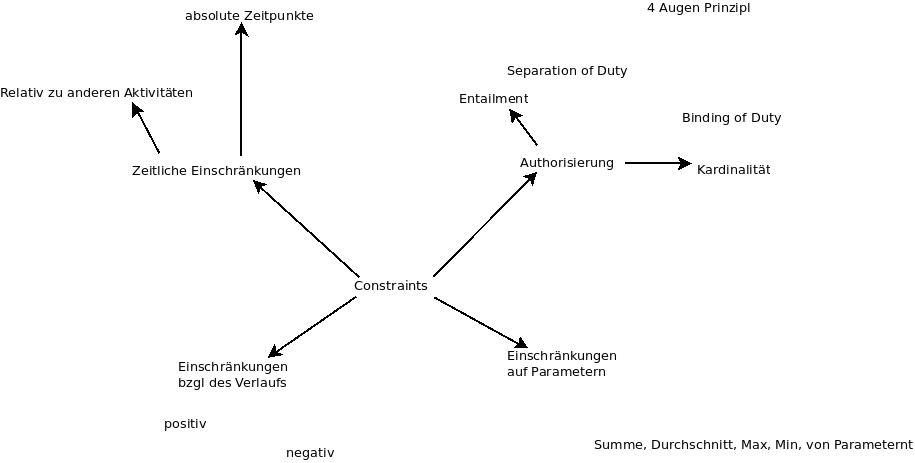
\includegraphics[width=0.9\textwidth]{Figures/Constraints}
	\caption{Typen von Einschränkungen und regeln}
	\label{fig:constraints}
\end{figure}

\textbf{Sich gegenseitig ausschließende Tasks (Conflicting Tasks)}
TODO: kommt das zur Constraint Sammlung?
In manchen Fällen kann man Tasks nicht verschiedenen Rollen zuweisen  ohne die exisitierenden Rollen derart zu segmentieren, dass die schwer zu verwalten sind in Bezug auf das organsiatorische Modell. Außerdem können Rollenhierarchien dazu verwendet werden, in zwei verschiedenen Rollen zu agieren, die eigentlich getrennt waren. ZB könnte ein Manager als ein Clerk und gleichzeitig als sein eigenener Supervisor handeln.\\
Deswegen definieren wir \textbf{TC} $\subset$ T als eine Menge von \textbf{kollidierenden Tasks}. TC beinhaltet Tasks, deren Allokation von der Allokation von vorhergehend ausgeführten Tasks aus TC abhängt. Diese Abhängigkeit wird als Abhängigkeit zwischen Tasks aus TC beschrieben. $t_c\in TC$ gilt als entailed Task von $t_m\in TC$, wenn die Allokation von $t_n$ von der Allokation von $t_m$ eingeschränkt wird, mit $t_m<t_n$.
\cite{wolter_modeling_of_TBAC_in_BPMN}\\

\textbf{Zeitliche Beschränkungen}\\
--absolute Einschränkungen\\
Das sind Einschränkungen, die sich auf einen absoluten Zeitpunkt beziehen, wie zum Beispiel dass besondere Kredite nicht mehr vergeben werden dürfen, nachdem das Angebot erloschen ist. Sollte nach dem festgelegten Datum trotzdem dieser Kredit vergeben werden, stellt das einen Regelbruch dar.
--relative Einschränkungen\\
Relative Einschränkungen beziehen sich auf vorher erfüllte Aufgaben und schränken die weiteren für einen bestimmten Zeitraum ein.\\

\textbf{Einschränkungen auf Parametern}\\
Einschränkungen, die mit der Akkumulation von Aktivitäten arbeiten, geben oft eine Grenze für einen Parameter in einem bestimmten Zeitraum vor. Diese Art der Einschränkungen ist oft mit zeitlichen Einschränkungen verbunden.\\

\textbf{Entailment Constraint}
c=(TC, $n_u$,$m_{th}$) mit $n_u$ als minimale Anzahl an verschiedenen Usern, die einem Task zugewiesen werden müssen. Wenn $t_{ki}$ eine Instanz des Tasks $t_k$ ist, dann ist $m_th$ der Grenzwert von der Summe der Task Instanzen, denen ein User zugewiesen sein darf.
\cite{wolter_modeling_of_TBAC_in_BPMN}
\textbf{Separation of Duty}\\
...\\
\textbf{Binding of Duty Constraints}\\
...\\
\textbf{Cardinality Constraints}\\
..\\
\textbf{Workflow Soundness}\\
Das sind Regeln, die allgemein den korrekten Ablauf eines Prozesses sicherstellen sollen. Diese Regeln beziehen sich im Allgemeinen nicht darauf, welcher Nutzer eine Aktivität ausgeführt hat (keine Authorisierungs-Einschränkungen) sondern betrachten die Tatsache, ob eine Aktivität zu einem korrekten Zeitpunkt oder in einem korrekten Zusammenhang ausgeführt wurde.

TODO Zum ein oder anderen Vielleicht Quellenangabe

\subsection{Gültigkeitsbereich von Constraints}
//TODO Welche der Einschränkungen gehört wohin
\textbf{Intra-Instanz}\\
Die meisten Ansätze beziehen sich auf Regeln, die in Bezug zu einer Prozessinstanz stehen. Hier gilt, dass die Prozessinstanz für alle Aktivitäten die selbe ist. Sollten zwei Aktivitäten zu verschiedenen Instanzen gehören, werden sie nicht gegeneinander betrachtet. Seien A und B zwei Aktivitäten, dann gilt A.caseID = B.caseID. 
\\
\textbf{Inter Instanz}\\
Wie bereits erkannt wurde, reicht es nicht aus, nur Einschränkungen innerhalb eines Prozesses zu definieren, da sich eine kriminelle Handlung auch über mehrere Instanzen bemerkbar machen kann. TODO Weitere Erklärung oder kleineres Beispiel. Die Einschränkung von oben wird hier aufgehoben, es gilt jedoch noch, dass die betrachteten Tasks zum selben Prozessschema gehören müssen, dh A.case = B.case
\\
\textbf{Inter-Prozess}\\
Die Regeln beziehen sich auf alle Aktivitäten, unabhängig davon, zu welcher Prozessinstanz oder welchem Prozessschema sie gehören. Diese Einschränkungen betrachten häufig die Akkumulation von verschiedenen Aktivitäten, ihre Anzahl bzw Operationen auf die Aggregation ihrer Parameter.


% Chapter Template

\chapter{Praxis} % Main chapter title

\label{Chapter5} % Change X to a consecutive number; for referencing this chapter elsewhere, use \ref{ChapterX}

\lhead{Chapter 5. \emph{Ergebnisse}} % Change X to a consecutive number; this is for the header on each page - perhaps a shortened title

%----------------------------------------------------------------------------------------
%	PRAXIS
%----------------------------------------------------------------------------------------

\section{Implementierung}

\subsection{Aufbau mein Programm}

\begin{figure}[ht]
	\centering
  \includegraphics[width=0.9\textwidth]{"Figures/myProg"}
	\caption{Aufbau mein Programm}
	\label{fig: myprog}
\end{figure}

Das Programm liest mittels SEWOL MXML logs ein und übersetzt sie in Status Prädikate. 
Die Constraints werden ebenfalls eingelesen und in Regelprädikate übersetzt. Der Parser für die Grammatik wurde mit ANTLR\cite{antlr} erzeugt.
Die eigentliche Untersuchung kann entweder durch ein Skript oder innerhalb des Javacodes gestartet werden.

\subsection{Wissensbasis}
Die Wissensbasis wird aus den Logs herausgelesen und in entsprechende Prädikate übersetzt. Auf Basis dieser Prädikate arbeitet der Modelchecker. Die Wissensbasis besteht aus genau 7 möglichen Prädikaten, welche ausreichen, um die Events vollständig wiederzugeben:\\

\begin{enumerate}
\item \textbf{workflow{\_}name(caseID, workflowName)}: Weist einer Case ID einen eindeutigen Namen hinzu, welcher der Workflow Spezifikation entspricht. Die Case ID kennzeichnet die Instanz, konkrete Ausführung eines Workflows. Dieses Prädikat dient jedoch nur zur Vollständigkeit. Sollte es für den Arbeitsablauf keinen eindeutigen Namen geben, wird dieses Prädikat nicht gesetzt. Es kann im Modelchecker dann auch nicht darauf zugegriffen werden.
\item \textbf{activity{\_}workflow(activityID, caseID)}: Setzt fest, zu welcher case ID die Activity gehört. TaskID wird intern vom Transformer gesetzt.
\item \textbf{activity{\_}name(taskID, taskName)}: Legt den Namen der Activity fest. Dieser ist im MXML Modell als WorkflowModelElement zu finden.
\item \textbf{timestamp(taskID, timestamp in ms)}: Zeitpunkt der Aktivität in ms nach 1970. Sollte kein Zeitpunkt eingetragen sein, wird entweder kein Fakt gesetzt, oder es wird die Reihenfolge der Einträge genommen. Dazu wird der letzte Wert + 1 ms gesetzt.
\item \textbf{eventtype(taskID, eventtype)}: Der Eventtyp der Aktivität. Im Grundmodell sind es start, accept, abort, ... Kann jedoch varriieren.
\item \textbf{executed{\_}user(user, taskID)}: Der Nutzer, der die Activity ausgeführt hat.
\item \textbf{executed{\_}group(group, taskID)}: Die Rolle, in der die Activity ausgeführt wurde. Man beachte, dass ein Nutzer mehrere Rollen haben kann.
\item \textbf{task{\_}attribute(taskID, attrName, attrType, attrValue)}: In dieser Wissensbasis wird zwischen zwei Typen unterschieden. String-Attributen, welche nur Vergleichsoperatoren kennen. Hat das Attribut im ürsprünglichen Event ein anderes Format, muss es für die Analyse in eine passende String Darstellung konvertiert werden. 
\end{enumerate}

Die erste Zeile aus dem Eventlog aus Tabelle \ref{tab:examplelog} wird in folgende Wissensbasis konvertiert:
\begin{table}
\begin{tabular}{ccc}
activity{\_}workflow(0,0) & activity{\_}name(0,'Approach check') & timestamp(0, 123)\\ 
eventtype(0, start) & executed{\_}user(0, 'Mark') & executed{\_}role(0, 'Admin') 
\end{tabular}
\caption{fd}
\label{tab:knowledge}
\end{table}



TODO: Closed World, was passiert mit nicht angegebenen Zeiten,.

\subsection{Algorithmus}
Zuerst aus Logs Status-Prädikate auslesen.\\
Für jedes critical task pair entsprechende collaborateurs setzen.\\
Schleife über Regeln\\
--Die resultierenden Heads bestimmen und schauen, ob es für cannot do ein executed und für must do kein executed gibt-> dann wurde es verletzt. Um das herauszufinden, wird die Regel in executed $ - >$ blabla, oder not(executed) $- >$ blabla übersetzt.\\
 
Einfaches Beispiel: Rule: executed(ui, t1)-> cannot do(ui,t2) und status: executed('tom', t1). Daraus wird abgeleitet: cannot do('tom', t2). Da es nicht in der DB ist, ist alles OK
 
% Chapter Template

\chapter{Ergebnisse und Diskussion} % Main chapter title

\label{Chapter5} % Change X to a consecutive number; for referencing this chapter elsewhere, use \ref{ChapterX}

\lhead{Chapter 5. \emph{Ergebnisse}} % Change X to a consecutive number; this is for the header on each page - perhaps a shortened title
\section{Evaluation}
Sämtliche hier vorgestellte Regeln wurden mit speziell erstellen Logs in SEWOL erfolgreich getestet. Blabla Erklärung

Im Folgenden wird ein einfaches Beispiel vorgestellt und der genaue Ablauf der Auswertung besprochen.

\section{Diskussion}


Wie kann man die restlichen Constraints implementieren\\
Compliance Checking:\\
Cannot do und Must execute vergleichen.\\
Optimierung??\\
Weitere Enforcement Prädikate definieren




%\input{Chapters/Chapter6} 
%\input{Chapters/Chapter7} 

%----------------------------------------------------------------------------------------
%	THESIS CONTENT - APPENDICES
%----------------------------------------------------------------------------------------

\addtocontents{toc}{\vspace{2em}} % Add a gap in the Contents, for aesthetics

\appendix % Cue to tell LaTeX that the following 'chapters' are Appendices

% Include the appendices of the thesis as separate files from the Appendices folder
% Uncomment the lines as you write the Appendices

% Appendix A

\chapter{Weitere Beispiele für die Benutzung der Grammatik} % Main appendix title

\label{GrammatikBeispiele} % For referencing this appendix elsewhere, use \ref{AppendixA}

\lhead{Anhang A. \emph{Grammatik Beispiele}} % This is for the header on each page - perhaps a shortened title

zusätzliche Beispiele zu Constraints und deren Darstellung\\
\textbf{Intra Instance}\\

Task1 und Task2 dürfen nicht vom selben User ausgeführt werden\\
$- >$ IF USER executed 'Task1' THEN USER cannot execute 'Task2'\\

\textbf{Inter Instance}\\

\textbf{Inter Process}\\

% Appendix B

\chapter{Argumente und Konfiguration} % Main appendix title

\label{Argumente} % For referencing this appendix elsewhere, use \ref{AppendixA}

\lhead{Appendix B. \emph{Argumente und Konfiguration}} % This is for the header on each page - perhaps a shortened title

Input Dateien für die Constraints: Wo sind sie? Wie kann man mehrere einlesen? (Dadurch sollen die Regeln wiederverwendbar werden)\\
Kann man vielleicht eine textdatei anlegen, wo die Inputfiles drinstehen?
Input Dateien MXML - wo sind sie? Wird der ganze Ordner eingelesen oder gibt man ein bestimmtes File an?\\
Output Logger  - Konsole oder File. Einstellung Level\\
Unterscheiden zwischen Parser Logger und Visitor Logger?\\
Konfigurationsdatei für die vorkommenden Events\\
Output Ordner

\begin{table}[h]
  \centering
  \begin{tabular}{|c|c|c|c|}
  Parameter & Argument & Default & Beschreibung\\
  \hline
  --constraintfolder & abs oder rel Pfad zum Ordner & rulefiles & ..\\
  --logfolder &abs oder rel Pfad zum Ordner & logfiles & ..\\
  --outputfolder &abs oder rel Pfad zum Ordner &prologfiles & ..\\
  \end{tabular}
 Tabelle mit allen möglichen Parametern
  \caption{Kommandozeilenparameter}
  \label{tab:commandlineargs}
\end{table}

\input{"Appendices/Programm starten"}
% Appendix D

\chapter{Fehlermeldungen} % Main appendix title

\label{Fehlermeldungen} % For referencing this appendix elsewhere, use \ref{AppendixA}

\lhead{Appendix D. \emph{Fehlermeldungen}} % This is for the header on each page - perhaps a shortened title

Write your Appendix content here.

%\input{Appendices/AppendixC}

\addtocontents{toc}{\vspace{2em}} % Add a gap in the Contents, for aesthetics

\backmatter

%----------------------------------------------------------------------------------------
%	BIBLIOGRAPHY
%----------------------------------------------------------------------------------------

\label{Bibliography}

\lhead{\emph{Bibliography}} % Change the page header to say "Bibliography"

\bibliographystyle{unsrtnat} % Use the "unsrtnat" BibTeX style for formatting the Bibliography

\bibliography{Bibliography} % The references (bibliography) information are stored in the file named "Bibliography.bib"

\end{document}  
